\documentclass[a4paper]{article}

%% Language and font encodings
\usepackage[english]{babel}
\usepackage[utf8x]{inputenc}
\usepackage[T1]{fontenc}

%% Sets page size and margins
\usepackage[a4paper,top=3cm,bottom=2cm,left=3cm,right=3cm,marginparwidth=1.75cm]{geometry}

%% Useful packages
\usepackage{amsmath}
\usepackage{graphicx}
\usepackage[colorinlistoftodos]{todonotes}
\usepackage[colorlinks=true, allcolors=blue]{hyperref}

\title{Pick Up! SRP}
\author{Michael Chan (chanmic), Ryan Miura (miurary), \\Christopher Cooper (cooperchri), Jordan Clark (clarkj3), Ziyu Xiong (xiongz)}

\begin{document}
\maketitle

\section{Project Description}
Busy work schedules make it difficult for many adults to stay physically active. Sports are a great way to stay active however many working adults struggle to find people to play with that have similar availabilities. Creating the website Pick Up will help these people find other people to play sports with to stay active.  This website will allow people to post a sporting event and allow others to see this event and join it.

In the past, people that wanted to play a sport often went to the nearest park and hoped to join in a game there. Pick Up would allow people to find games during their availability and ensure that they can join a game.  Our implementation of Pick Up will allow users to find games with their availability with four main functionalities, user authentication, event listings, post filtering, and groups, to allow others to find people to play sports with to stay active. Additionally, stretch goals of the Pick Up would include, Google APIs for the specific location of users and creating mobile app platform of Pick Up.

User authentication is an essential functionality of the website to protect the identity of the users and ensure users authenticity to prevent fake or spam postings. Users will be asked to either create an account or log into their existing account. New yours that make an account will have to verify their authenticity by an email confirmation.

Event listings will be a running list of sports events coming up. People will be allowed to create a post of upcoming games for other users to see. The event post will be marked with a date of the event and will be cleared from the event listings when the date has past to ensure that all event listings are current and up to date.

Post filtering will allow users to filter down the even listings to show only the things they are interested in. Users will be given the option to select specific sports they are interested in, dates, time, location, and level of ability. These filters will allow users to see only event listings of sports they are interested in during times when they are available in their area.

Groups will help users better communicate with each other about the details of the event. If a user finds an even, they are interested in, and the creator of the event post allows them to be a player in the game they will be added to a group that has all the players in the upcoming event so that they can coordinate the specifics of the event.

Additionally, we will provide a question and answer page to help users better understand the website if they have any questions. Since Pick Up would be created as a website, this project will use HTML, CSS, JavaScript, nodejs, express, and MongoDB. None of these require anything more than a text editor (Putty, MobaXTerm, etc.) and access to the ENGR servers.

\begin{figure}
  \centering
		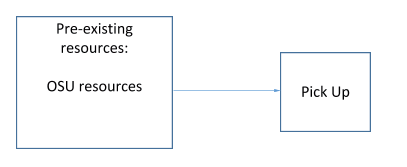
\includegraphics[width=.5\textwidth]{images/diagram.png}
	\caption{Pre-existing resources plugging into our approach.}
    \label{fig:diagram}
\end{figure}

\newpage

\section{Use Cases}

\subsection{User Authentication}

\textbf{Goal:} 
User information is stored and secured; the user will be able to access their information with identification (ID/Password).\\
\\
\textbf{Actor:} 
Applicant, coordinator\\ 
\\
\textbf{Preconditions:} 
\begin{itemize}
\item User is registered in the system
\item User has an ID and password and is at login screen.
\end{itemize}
\textbf{Postconditions:} 
\begin{itemize}
\item User will be able to post/search for listings, and is now enabled to send an application. 
\item The user will also be able to create/join groups and send/accept friend requests.
\end{itemize}
\textbf{Flow of events:} 
\begin{enumerate}
\item The user has registered their ID, password, and email address and the system has hashed the information and stored it. 
\item The user can now navigate to the login screen and log in to their account as long as they have their ID and password. 
\item If the user is unable to login, they're able to request to recover their ID/password by sending a verification link to their email. 
\item If the user is able to login, then an indicator (replacing the login button) is displayed to show that they're currently logged in. 
\item The user is now able to view/post event postings, create/join groups, send/accept friend requests, manage friends/groups, and change user settings. 
\end{enumerate}
\textbf{Quality requirements:} 
The user remembers ID, password, and email just in case. If the user cannot login then the user is limited to a number of logins, for example five, to prevent strain on the server from repetitive attempts.

\subsection{Post Event}

\textbf{Goal:} 
This allows the user to post event in the website under a specific category page. Additionally, all the information given by the user can be searched successfully by using search method to filter all the posts including the new post just added.\\
\\
\textbf{Actor:} 
Customers, website. If the customers clicking at the “adding events” button, the website will pop-up a small window asking the customers to complete the information of the event that he/she wants to start.\\ 
\\
\textbf{Preconditions:} 
\begin{itemize}
\item User is registered and signed in and is at the listings page and clicks "add event."
\end{itemize}
\textbf{Postconditions:} 
\begin{itemize}
\item The information from display to the screen asking customers to fill all the information about the event. After that, click a “post” button to close the window and send the information to our server.\newpage
\end{itemize}
\textbf{Flow of events:} 
\begin{enumerate}
\item The user logs in to the web page.
\item The user navigates to the event category page that they wish to add to.
\item The user clicks the "add event" button.
\item The user fills out the information in the form.
\item If the user doesn't fill out all the fields, the website will give an error message.
\item The user clicks the "post" button.
\end{enumerate}
\textbf{Quality requirements:} 
The given information be added to the server correctly. In other words, the new event just added can be searched by the filter successfully. 

\subsection{Search Events}

\textbf{Goal:}
Search events posted by other users on the site.\\
\\
\textbf{Actor:}
Event Applicant\\
\\
\textbf{Preconditions:}
\begin{itemize}
   \item User must have valid account.
   \item User must be at login screen.
\end{itemize}
\textbf{Postconditions:} 
\begin{itemize}
   \item System displays a list of events and potential filters.
\end{itemize}
\textbf{Flow of Events:}
\begin{enumerate}
   \item User enters username and password.
   \item System validates login credentials.
   \item System displays sports available for browsing.
   \item User selects desired sport from list.
   \item System displays events based on default filters, and all filter options.
\end{enumerate}
\textbf{Quality Requirements:}
System displays a maximum of 10 or 20 (user option) event postings at a single time.

\subsection{Use Case Selection Explained}
\textbf{User Authentication:} This is the main factor of nearly all use cases. Since this is a user-based website, a user authentication system is required to manage events, groups, and friends.\\
\\
\textbf{Post/Search Events:} 
The nature of the application at a very basic level is to post information about a planned event and for others to find that information to potentially join the event. With this in mind, two events must be capable of occuring within the system in order for the goal of the service to be met: posting information about an event, and searching for events that have been posted. 

While other features are desired for the system to be pleasing for users, they are not exactly needed. With these two use cases implemented and working, the service could provide a bare minimal functionality that would accomplish the intended goal. Without these two key usage scenarios, the site would have no content and thus no purpose.


\subsection{"Main" Errors}

\textbf{Error:}
User inputs incorrect username or password at the login screen.\\
\textbf{Solution:}
Check database for username and check the hashed password. If either fails, bring user back to login with a displayed error message that the username or password was incorrect.\\
\\
\textbf{Error:}
User inputs incomplete or incorrect information in event post.\\
\textbf{Solution:}
Check that all form fields have data entered and that any with specific format requirements match the regular expression. If either condition fails, return user to the html form page.\\
\\
\textbf{Error:}
User attempts to send message to nonexistent user.\\
\textbf{Solution:}
Check database for intended user before attempting to enter message into inbox database. Give error message to user and send them back to the message composition form.\\
\\
\textbf{Error:}
User attempts to apply to event/group that was deleted/removed since user's last refresh.
\textbf{Solution:}
When users are redirected to the event application form, check event ID requested. If the ID is not found, redirect user to event listing page and give error message that the event has expired or been removed by the posting user.

\section{Planning}
\subsection{Milestones/Tasks:}
\begin{enumerate}
\item Finish HTML: The base of the website is necessary for everything after.
\item Finish CSS: Transform the HTML into a user-friendly GUI. This is purely for appearance, so JS is unnecessary at this point time. However, they can be completed simultaneously.
\item Finish Javascript: Gives the HTML functionality, allowing the user to navigate to different aspects of the website.
\item Finish server (Node.js): Allows the user to access the website.
\item Finish database (MongoDB): Stores user data. Although this will be the key aspect of the Pick Up! it's only possible to set this up after the server is up and running.
\end{enumerate}
We'll need to use the OSU servers to avoid purchasing domains to host the website.
\newpage
\subsection{Schedule/Timeline:}
\begin{figure}[!ht]
  \centering
		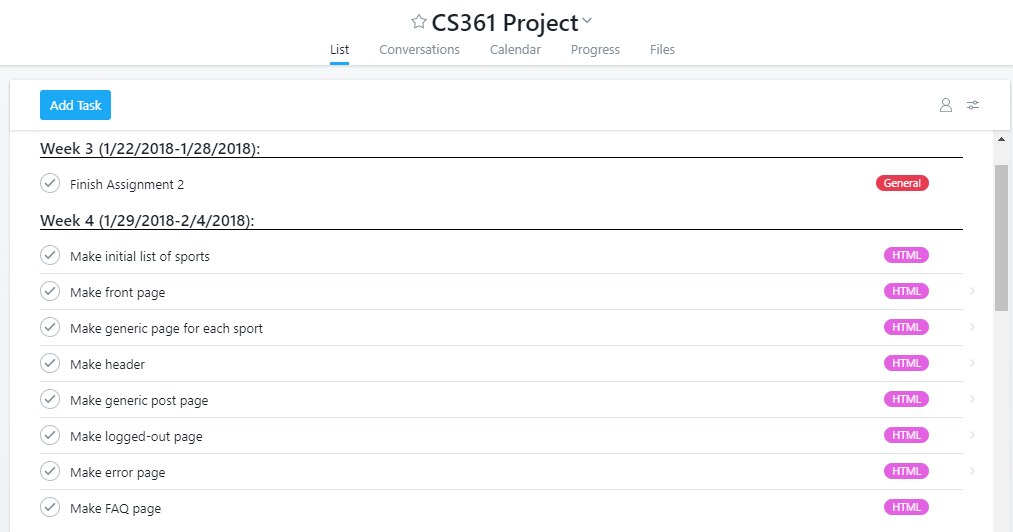
\includegraphics[width=1\textwidth]{images/sched1.png}
    \label{fig:sched1}
\end{figure}
\begin{figure}[!ht]
  \centering
		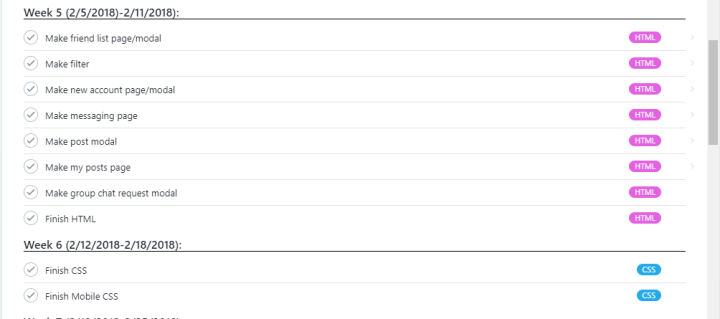
\includegraphics[width=1\textwidth]{images/sched2.png}
    \label{fig:sched2}
\end{figure}
\begin{figure}[!ht]
  \centering
		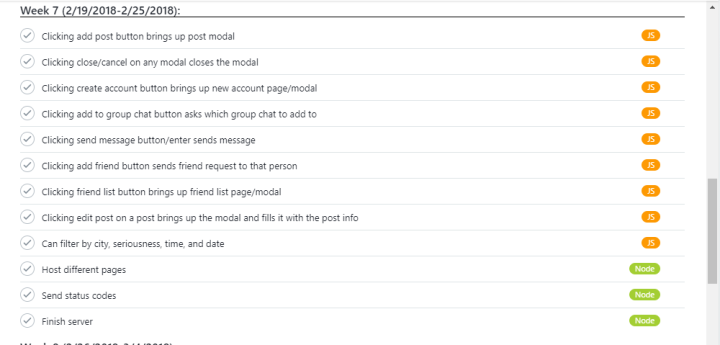
\includegraphics[width=1\textwidth]{images/sched3.png}
    \label{fig:sched3}
\end{figure}
\begin{figure}[!ht]
  \centering
		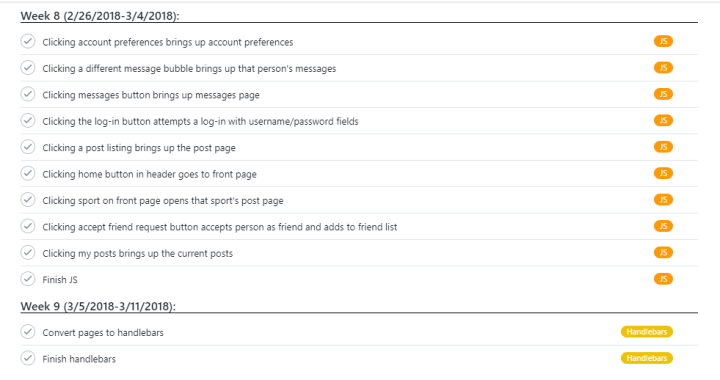
\includegraphics[width=1\textwidth]{images/sched4.png}
    \label{fig:sched4}
\end{figure}
\begin{figure}[!ht]
  \centering
		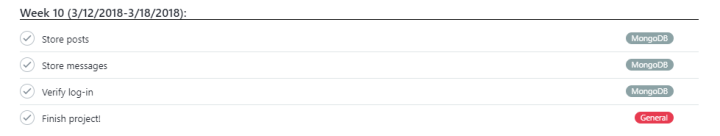
\includegraphics[width=1\textwidth]{images/sched5.png}
        \caption{Schedule formed in Asana}
    \label{fig:sched5}
\end{figure}
\newpage
\begin{flushleft}
\subsection{Project Tracking:} We’ve decided to use Asana to track out progress. Since we are building a website, I structured it much like our progression on CS290. I’ve also split the tasks into weeks, so it shouldn’t be an overload of stuff. This schedule will probably change once we meet and design further.
\end{flushleft}

\begin{flushleft}
\subsection{Risk Management:}
All of these risks are things that are outside of what we have done in the past through classes at OSU.
\begin{itemize}
\item Sending friend requests
This poses a threat due to the complexity of the interaction. Requesting to be someone’s friend sends a request to that person and lets the user know a request has been sent. The requested user can either accept or decline it. This communication between two accounts seems a bit complex and can get easily messed up. By sitting down with our team and flushing out a design for how exactly we will accomplish this task, we can minimize the risk as much as possible.
\item User authentification
Storing the username and password of each user and verifying them via hash seems like it could require a bit of effort, but writing it now seems very easy. Simply hash and store it the first time in MongoDB, then rehash upon log-in. It sounds easy, but we’ve never tried it so I still feel it’s worth to list as a risk. Testing this approach won’t take too much time, so I think that will be the best way to see if it works. 
\item Group chat requests
This risk is along the same lines as the friend request one. It functions in almost the exact same way. Taking the time to flush out the system will cut down the risk, and once one works then both will work.
\item Storing posts/messages
This is risky because we have to store the messages with the same hash for a user so their messages come up and not someone else’s. Storing posts is easy as it’s something we have done before. Again, I think flushing out our design for this feature will cut down the risk and make it easy to implement.
\item Overplanning
Adding more features than our time frame can handle is a risk we will have to address. We are going to meet this week to deeply design our product, so I think by doing this we will minimize the risk of randomly adding in more features because we will have the time to get it all out before we actually start coding.
\end{itemize}
\end{flushleft}

\subsection{Meeting Report:}
This week the group was able to meet twice. The first meeting took place briefly after Thursday's lecture. During this meeting, everyone introduced themselves and we discussed a time and meeting place to meet again to go into more detail of the assignment. We agreed to meet on Saturday at the library at 1:00 pm.

During the second meeting this week, as a group we discussed to project in greater detail and split up the work for this week’s assignment. Jordan worked on the project description, Michael, Ziyu, and Christopher worked on the use cases, each focusing on one use case, Ryan worked on the planning, and Jordan worked on the meeting report. 

While each person was assigned a specific task, the group still worked collaboratively throughout the meeting asking each other for help, points of clarifications, and discussed other ideas for the project. Through the collaboration of the meeting, the group got a better understating of the design and applications of the project. Additionally, the team was very flexible with ideas and was able too able to discusses changes to the project and additional applications that were not in the original vision statement proposal. 

At 3:45 pm the group finished the meeting with a good understating on their part of this week’s assignment and the project as a whole. Everyone agreed to have their part of the assignment finished by Monday morning the latest at which time Michael will make the final pdf to submit. 

The group plans to meet this Wednesday again at 8:00 pm in the library to discuss the design planes in greater detail and figure out how to break down the next assignment.   



\end{document}